\documentclass[aspectratio=169,11pt]{beamer}
\usepackage{amsmath,amssymb}
\usepackage{booktabs}
\usepackage{tikz}
\usepackage[T1]{fontenc}
\usepackage{lmodern}

\definecolor{courseblue}{RGB}{0,91,155}
\definecolor{courseorange}{RGB}{190,72,20}
\setbeamercolor{structure}{fg=courseblue}
\setbeamercolor{frametitle}{fg=courseblue}
\setbeamercolor{alerted text}{fg=courseorange}
\setbeamertemplate{navigation symbols}{}
\setbeamertemplate{footline}[frame number]
\setbeamertemplate{itemize items}[circle]

\title{Slice sampling}
\subtitle{The sampling identity, the algorithm, and why it works}
\author{Econometrics 32706}
\date{}

\begin{document}

\begin{frame}
  \titlepage
\end{frame}

\begin{frame}{The problem}
  We want draws from a density known only up to a normalizing constant:
  \[
    \pi(x)=\frac{q(x)}{Z},
    \qquad
    Z=\int_{\mathbb R}q(t)\,dt.
  \]
  We can evaluate \(q(x)\), but calculating \(Z\) or sampling
  directly from \(\pi\) may be difficult.
  \vspace{0.7em}

  \alert{Key idea:} represent \(\pi\) as the marginal distribution
  of a point chosen uniformly from a region under the graph of \(q\).
  This representation leads to slice sampling.
\end{frame}

\begin{frame}{Proposition: uniform sampling under a graph}
  Let \(q:\mathbb R\to[0,\infty)\) be measurable and
  \(0<Z=\int_{\mathbb R}q(x)\,dx<\infty\). Define
  \[
    A=\{(x,h)\in\mathbb R\times(0,\infty):0<h<q(x)\}.
  \]
  \begin{block}{Sampling proposition}
    If \((X,H)\) is uniform on \(A\) with respect to area,
    then \(X\) has density
    \[
      \pi(x)=\frac{q(x)}{Z}.
    \]
  \end{block}
  \vspace{0.5em}
  The height \(H\) is auxiliary: discard it after sampling
  \((X,H)\), and the remaining \(X\) follows the target distribution.
  \vspace{0.55em}

  {\tiny Source: Neal (2003), \emph{Slice sampling},
  \emph{Annals of Statistics} 31(3), 705--767,
  \href{https://doi.org/10.1214/aos/1056562461}{doi:10.1214/aos/1056562461}.}
\end{frame}

\begin{frame}{Proof of the sampling proposition}
  Adding vertical strips of height \(q(x)\) (Tonelli's theorem) gives
  \[
    |A|=\int_{\mathbb R}\int_0^{q(x)}dh\,dx
       =\int_{\mathbb R}q(x)\,dx=Z.
  \]
  \alert{Thus, the area of \(A\) is \(Z\).}
  \vspace{0.25em}

  Define a uniform density on \(A\):
  \[
    p(x,h)=\frac{1}{|A|}\mathbf 1\{(x,h)\in A\}
          =\frac{1}{Z}\mathbf 1\{0<h<q(x)\}.
  \]
  Its marginal density for \(X\) is \(\pi\):
  \[
    p_X(x)=\int_0^{q(x)}\frac{1}{Z}\,dh
          =\frac{q(x)}{Z}=\pi(x).
  \]
  \alert{Conclusion:} sample \((X,H)\) from this joint density
  and keep only \(X\); then \(X\sim\pi\).
\end{frame}

\begin{frame}{Conditional 1: the height given the position}
  From slide 4,
  \[
    p(x,h)=\frac{1}{Z}\mathbf 1\{0<h<q(x)\},
    \qquad p_X(x)=\frac{q(x)}{Z}.
  \]
  For a fixed \(x\) with \(q(x)>0\), divide the joint density
  by the marginal density of \(X\):
  \[
    \begin{aligned}
      p(h\mid x)
      &=\frac{p(x,h)}{p_X(x)}\\
      &=\frac{1}{q(x)}\mathbf 1\{0<h<q(x)\}.
    \end{aligned}
  \]
  This is constant on the vertical interval \((0,q(x))\), so
  \[
    H\mid X=x\sim U(0,q(x)).
  \]
\end{frame}

\begin{frame}{Why the height marginal contains \(|S_h|\)}
  Fix a height \(h>0\). The horizontal slice is
  \(S_h=\{x:q(x)>h\}\); let \(|S_h|\) be its total length.
  \vspace{0.4em}

  At this height, the joint density is \(1/Z\) for every
  \(x\in S_h\), and zero for every \(x\notin S_h\):
  \[
    p(x,h)=\frac{1}{Z}\mathbf 1\{x\in S_h\}.
  \]
  To find the marginal density of \(H\), add the joint density
  over all possible positions:
  \[
    \begin{aligned}
      p_H(h)
      &=\int_{\mathbb R}p(x,h)\,dx
       =\int_{S_h}\frac{1}{Z}\,dx\\
      &=\frac{1}{Z}\,|S_h|.
    \end{aligned}
  \]
  \alert{Intuition:} the longer the horizontal slice at \(h\),
  the more area of \(A\) lies near that height.
\end{frame}

\begin{frame}{Conditional 2: the position given the height}
  By definition \(S_h=\{z:q(z)>h\}\). For a fixed \(h>0\),
  \[
    x\in S_h\quad\Longleftrightarrow\quad q(x)>h
      \quad\Longleftrightarrow\quad 0<h<q(x).
  \]
  The two indicators therefore agree. The joint density on slide 4
  can be written, for \(h>0\), as
  \[
    p(x,h)=\frac{1}{Z}\mathbf 1\{0<h<q(x)\}
          =\frac{1}{Z}\mathbf 1\{x\in S_h\}.
  \]
  We also showed \(p_H(h)=|S_h|/Z\) when \(|S_h|>0\).
  Divide the joint density by this height marginal:
  \[
    \begin{aligned}
      p(x\mid h)
      &=\frac{p(x,h)}{p_H(h)}\\
      &=\frac{1}{|S_h|}\mathbf 1\{x\in S_h\}.
    \end{aligned}
  \]
  Thus every position in \(S_h\) has the same conditional density,
  and positions outside it have density zero:
  \[
    X\mid H=h\sim U(S_h).
  \]
\end{frame}

\begin{frame}{How to use it}
  The joint law has two conditional distributions:
  \[
    h\mid x\sim U(0,q(x)),
    \qquad
    x\mid h\sim U(S_h).
  \]
  \begin{center}
    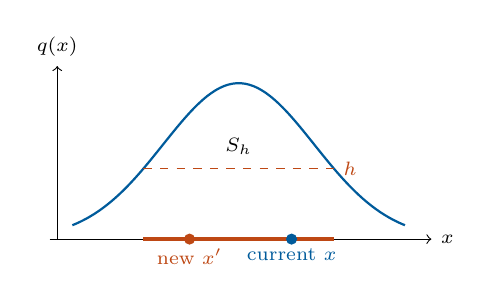
\begin{tikzpicture}[x=0.96cm,y=1.98cm,
                        every node/.style={font=\scriptsize}]
      \draw[->] (-2.5,0)--(2.55,0) node[right] {\(x\)};
      \draw[->] (-2.4,0)--(-2.4,1.11) node[above] {\(q(x)\)};
      \draw[courseblue,thick]
        plot[domain=-2.2:2.2,samples=80] (\x,{exp(-\x*\x/2)});
      \draw[courseorange,dashed] (-1.26,0.45)--(1.26,0.45)
        node[right] {\(h\)};
      \draw[courseorange,very thick] (-1.26,0)--(1.26,0);
      \fill[courseblue] (0.7,0) circle (2pt)
        node[below] {current \(x\)};
      \fill[courseorange] (-0.65,0) circle (2pt)
        node[below] {new \(x'\)};
      \node[above] at (0,0.48) {\(S_h\)};
    \end{tikzpicture}
  \end{center}
  The slice \(S_h\) contains every position whose density exceeds
  the chosen height.
  \vspace{0.25em}

  \alert{Alternate draws} from \(H\mid X\) and
  \(X\mid H\). This constructs a Markov chain whose stationary
  joint law is uniform on \(A\).
\end{frame}

\begin{frame}{The ideal slice-sampling update}
  Starting from the current position \(x\):
  \begin{enumerate}
    \setlength{\itemsep}{0.65em}
    \item Draw \(u\sim U(0,1)\), then set \(h=u\,q(x)\).
    \item Find the horizontal slice \(S_h=\{z:q(z)>h\}\).
    \item Draw \(x'\) uniformly from \(S_h\).
    \item Use \(x'\) as the next state and repeat.
  \end{enumerate}
  \vspace{0.6em}

  Since \(h<q(x)\), the current position always lies in the slice.
  A new height is drawn on every update, so the set of possible
  moves changes with the current state.
\end{frame}

\begin{frame}{A simple numerical example}
  Let \(q(x)=e^{-x^2/2}\), the standard normal kernel, and
  suppose the current position is \(x=1\).
  If the random draw is \(u=\tfrac12\), then
  \[
    h=u\,q(1)=\tfrac12 e^{-1/2}.
  \]
  The slice condition is
  \[
    e^{-z^2/2}>\tfrac12e^{-1/2}
    \quad\Longleftrightarrow\quad
    |z|<\sqrt{1+2\log 2}\approx 1.54.
  \]
  Thus \(S_h\approx(-1.54,1.54)\), and the ideal update draws
  \(x'\) uniformly from this interval.
  \vspace{0.45em}

  The example illustrates one possible height; the next update
  draws a new one.
\end{frame}

\begin{frame}{Why the update targets \(\pi\)}
  Both steps sample from conditionals of the \emph{same} joint law:
  \[
    x\ \xrightarrow{\ h\mid x\ }\ (x,h)\
      \xrightarrow{\ x'\mid h\ }\ (x',h).
  \]
  If \(x\sim\pi\), the first draw gives \((x,h)\sim p(x,h)\).
  The second conditional draw leaves that joint law unchanged.
  Discarding \(h\) therefore gives \(x'\sim\pi\).
  \vspace{0.75em}

  \alert{This is a Gibbs-sampling argument.} It proves that \(\pi\)
  is stationary for the update; successive states need not be
  independent.
  \vspace{0.4em}

  Another intuition: high-density points occur on many possible
  slices, so they receive more probability in the long run.
\end{frame}

\begin{frame}{When the slice is hard to sample from}
  The ideal update assumes we can draw uniformly from \(S_h\).
  For a complicated density, its endpoints may be unknown and
  \(S_h\) may have several pieces.
  \vspace{0.55em}

  A practical one-dimensional slice sampler constructs a bracket
  around the current point, tests candidate positions, and shrinks
  the bracket after rejections. The bracket rules must preserve the
  correct conditional distribution on the slice.
  \vspace{0.65em}

  The height step remains \(h=u\,q(x)\). If we work with log densities,
  the equivalent threshold is
  \[
    \log h=\log q(x)+\log u.
  \]
  This form avoids evaluating a tiny density value directly.
\end{frame}

\begin{frame}{What to remember}
  \begin{enumerate}
    \setlength{\itemsep}{0.8em}
    \item Uniform sampling under an unnormalized density curve
          gives the desired marginal distribution.
    \item A random height selects a horizontal slice; the position
          update moves within that slice.
    \item Alternating these conditional updates preserves the joint
          law and therefore the target marginal.
  \end{enumerate}
  \vspace{0.5em}

  {\small Reference: Radford M. Neal (2003),
  \emph{Slice sampling}, \emph{Annals of Statistics}
  31(3), 705--767,
  \href{https://doi.org/10.1214/aos/1056562461}{doi:10.1214/aos/1056562461}.}
\end{frame}

\end{document}
